\documentclass[]{article}
\usepackage{lmodern}
\usepackage{amssymb,amsmath}
\usepackage{ifxetex,ifluatex}
\usepackage{fixltx2e} % provides \textsubscript
\ifnum 0\ifxetex 1\fi\ifluatex 1\fi=0 % if pdftex
  \usepackage[T1]{fontenc}
  \usepackage[utf8]{inputenc}
\else % if luatex or xelatex
  \ifxetex
    \usepackage{mathspec}
  \else
    \usepackage{fontspec}
  \fi
  \defaultfontfeatures{Ligatures=TeX,Scale=MatchLowercase}
\fi
% use upquote if available, for straight quotes in verbatim environments
\IfFileExists{upquote.sty}{\usepackage{upquote}}{}
% use microtype if available
\IfFileExists{microtype.sty}{%
\usepackage{microtype}
\UseMicrotypeSet[protrusion]{basicmath} % disable protrusion for tt fonts
}{}
\usepackage[margin=1in]{geometry}
\usepackage{hyperref}
\hypersetup{unicode=true,
            pdftitle={Analysis of},
            pdfborder={0 0 0},
            breaklinks=true}
\urlstyle{same}  % don't use monospace font for urls
\usepackage{color}
\usepackage{fancyvrb}
\newcommand{\VerbBar}{|}
\newcommand{\VERB}{\Verb[commandchars=\\\{\}]}
\DefineVerbatimEnvironment{Highlighting}{Verbatim}{commandchars=\\\{\}}
% Add ',fontsize=\small' for more characters per line
\usepackage{framed}
\definecolor{shadecolor}{RGB}{248,248,248}
\newenvironment{Shaded}{\begin{snugshade}}{\end{snugshade}}
\newcommand{\KeywordTok}[1]{\textcolor[rgb]{0.13,0.29,0.53}{\textbf{#1}}}
\newcommand{\DataTypeTok}[1]{\textcolor[rgb]{0.13,0.29,0.53}{#1}}
\newcommand{\DecValTok}[1]{\textcolor[rgb]{0.00,0.00,0.81}{#1}}
\newcommand{\BaseNTok}[1]{\textcolor[rgb]{0.00,0.00,0.81}{#1}}
\newcommand{\FloatTok}[1]{\textcolor[rgb]{0.00,0.00,0.81}{#1}}
\newcommand{\ConstantTok}[1]{\textcolor[rgb]{0.00,0.00,0.00}{#1}}
\newcommand{\CharTok}[1]{\textcolor[rgb]{0.31,0.60,0.02}{#1}}
\newcommand{\SpecialCharTok}[1]{\textcolor[rgb]{0.00,0.00,0.00}{#1}}
\newcommand{\StringTok}[1]{\textcolor[rgb]{0.31,0.60,0.02}{#1}}
\newcommand{\VerbatimStringTok}[1]{\textcolor[rgb]{0.31,0.60,0.02}{#1}}
\newcommand{\SpecialStringTok}[1]{\textcolor[rgb]{0.31,0.60,0.02}{#1}}
\newcommand{\ImportTok}[1]{#1}
\newcommand{\CommentTok}[1]{\textcolor[rgb]{0.56,0.35,0.01}{\textit{#1}}}
\newcommand{\DocumentationTok}[1]{\textcolor[rgb]{0.56,0.35,0.01}{\textbf{\textit{#1}}}}
\newcommand{\AnnotationTok}[1]{\textcolor[rgb]{0.56,0.35,0.01}{\textbf{\textit{#1}}}}
\newcommand{\CommentVarTok}[1]{\textcolor[rgb]{0.56,0.35,0.01}{\textbf{\textit{#1}}}}
\newcommand{\OtherTok}[1]{\textcolor[rgb]{0.56,0.35,0.01}{#1}}
\newcommand{\FunctionTok}[1]{\textcolor[rgb]{0.00,0.00,0.00}{#1}}
\newcommand{\VariableTok}[1]{\textcolor[rgb]{0.00,0.00,0.00}{#1}}
\newcommand{\ControlFlowTok}[1]{\textcolor[rgb]{0.13,0.29,0.53}{\textbf{#1}}}
\newcommand{\OperatorTok}[1]{\textcolor[rgb]{0.81,0.36,0.00}{\textbf{#1}}}
\newcommand{\BuiltInTok}[1]{#1}
\newcommand{\ExtensionTok}[1]{#1}
\newcommand{\PreprocessorTok}[1]{\textcolor[rgb]{0.56,0.35,0.01}{\textit{#1}}}
\newcommand{\AttributeTok}[1]{\textcolor[rgb]{0.77,0.63,0.00}{#1}}
\newcommand{\RegionMarkerTok}[1]{#1}
\newcommand{\InformationTok}[1]{\textcolor[rgb]{0.56,0.35,0.01}{\textbf{\textit{#1}}}}
\newcommand{\WarningTok}[1]{\textcolor[rgb]{0.56,0.35,0.01}{\textbf{\textit{#1}}}}
\newcommand{\AlertTok}[1]{\textcolor[rgb]{0.94,0.16,0.16}{#1}}
\newcommand{\ErrorTok}[1]{\textcolor[rgb]{0.64,0.00,0.00}{\textbf{#1}}}
\newcommand{\NormalTok}[1]{#1}
\usepackage{longtable,booktabs}
\usepackage{graphicx,grffile}
\makeatletter
\def\maxwidth{\ifdim\Gin@nat@width>\linewidth\linewidth\else\Gin@nat@width\fi}
\def\maxheight{\ifdim\Gin@nat@height>\textheight\textheight\else\Gin@nat@height\fi}
\makeatother
% Scale images if necessary, so that they will not overflow the page
% margins by default, and it is still possible to overwrite the defaults
% using explicit options in \includegraphics[width, height, ...]{}
\setkeys{Gin}{width=\maxwidth,height=\maxheight,keepaspectratio}
\IfFileExists{parskip.sty}{%
\usepackage{parskip}
}{% else
\setlength{\parindent}{0pt}
\setlength{\parskip}{6pt plus 2pt minus 1pt}
}
\setlength{\emergencystretch}{3em}  % prevent overfull lines
\providecommand{\tightlist}{%
  \setlength{\itemsep}{0pt}\setlength{\parskip}{0pt}}
\setcounter{secnumdepth}{0}
% Redefines (sub)paragraphs to behave more like sections
\ifx\paragraph\undefined\else
\let\oldparagraph\paragraph
\renewcommand{\paragraph}[1]{\oldparagraph{#1}\mbox{}}
\fi
\ifx\subparagraph\undefined\else
\let\oldsubparagraph\subparagraph
\renewcommand{\subparagraph}[1]{\oldsubparagraph{#1}\mbox{}}
\fi

%%% Use protect on footnotes to avoid problems with footnotes in titles
\let\rmarkdownfootnote\footnote%
\def\footnote{\protect\rmarkdownfootnote}

%%% Change title format to be more compact
\usepackage{titling}

% Create subtitle command for use in maketitle
\newcommand{\subtitle}[1]{
  \posttitle{
    \begin{center}\large#1\end{center}
    }
}

\setlength{\droptitle}{-2em}
  \title{Analysis of}
  \pretitle{\vspace{\droptitle}\centering\huge}
  \posttitle{\par}
  \author{}
  \preauthor{}\postauthor{}
  \predate{\centering\large\emph}
  \postdate{\par}
  \date{June 23, 2018}

\usepackage{amsmath}
\usepackage{mathtools}
\usepackage{float}
\usepackage{xcolor,pifont}
\newcommand{\cmark}{\Large\textcolor{green}{\ding{52}}}
\newcommand{\xmark}{\Large\textcolor{red}{\ding{55}}}

\begin{document}
\maketitle

\newenvironment{sciabstract}{%
\begin{quote} \bf}
{\end{quote}}

\begin{verbatim}
## Loading required package: dplyr
\end{verbatim}

\begin{verbatim}
## 
## Attaching package: 'dplyr'
\end{verbatim}

\begin{verbatim}
## The following objects are masked from 'package:stats':
## 
##     filter, lag
\end{verbatim}

\begin{verbatim}
## The following objects are masked from 'package:base':
## 
##     intersect, setdiff, setequal, union
\end{verbatim}

\begin{verbatim}
## Loading required package: tidyr
\end{verbatim}

\begin{verbatim}
## Loading required package: knitr
\end{verbatim}

\begin{verbatim}
## Loading required package: ggplot2
\end{verbatim}

\begin{verbatim}
## Loading required package: maps
\end{verbatim}

\begin{verbatim}
## Loading required package: RColorBrewer
\end{verbatim}

\begin{verbatim}
## Loading required package: summarytools
\end{verbatim}

\begin{verbatim}
## Loading required package: magrittr
\end{verbatim}

\begin{verbatim}
## 
## Attaching package: 'magrittr'
\end{verbatim}

\begin{verbatim}
## The following object is masked from 'package:tidyr':
## 
##     extract
\end{verbatim}

\begin{verbatim}
## Loading required package: stargazer
\end{verbatim}

\begin{verbatim}
## 
## Please cite as:
\end{verbatim}

\begin{verbatim}
##  Hlavac, Marek (2015). stargazer: Well-Formatted Regression and Summary Statistics Tables.
\end{verbatim}

\begin{verbatim}
##  R package version 5.2. http://CRAN.R-project.org/package=stargazer
\end{verbatim}

\subsection{Import Breweries Data}\label{import-breweries-data}

\begin{Shaded}
\begin{Highlighting}[]
\CommentTok{#import breweries data}
\NormalTok{breweries_data <-}\StringTok{ }\KeywordTok{read.csv}\NormalTok{(}\StringTok{"../data/Breweries.csv"}\NormalTok{, }\DataTypeTok{header=}\OtherTok{TRUE}\NormalTok{)}

\CommentTok{#TODO: all columns to lowercase}
\CommentTok{#colnames(breweries_data) %<>% tolower # column names to lower case. %<>% is a compound operator that also reassigns the new column names back to the input dataframe}


\CommentTok{#summary of breweries raw data}
\NormalTok{brewery_summary_raw <-}\StringTok{ }\KeywordTok{select}\NormalTok{(breweries_data, State, Brew_ID) }\OperatorTok\StringTok{ }\CommentTok{#select columns}
\StringTok{                   }\NormalTok{dplyr}\OperatorTok{::}\KeywordTok{group_by}\NormalTok{(State) }\OperatorTok\StringTok{ }\CommentTok{#group by}
\StringTok{                   }\NormalTok{dplyr}\OperatorTok{::}\KeywordTok{summarize_all}\NormalTok{(}\KeywordTok{funs}\NormalTok{(}\DataTypeTok{count=}\KeywordTok{n_distinct}\NormalTok{(.), }\KeywordTok{min}\NormalTok{(.), }\KeywordTok{max}\NormalTok{(.), }\KeywordTok{mean}\NormalTok{(.), }\KeywordTok{median}\NormalTok{(.), }\KeywordTok{sd}\NormalTok{(.))) }\CommentTok{#specify aggregates to include in summary. (.) is a dummy variable}



\CommentTok{#print the summary in a way that it doesn't look like vomit}
\KeywordTok{kable}\NormalTok{(brewery_summary_raw, }\DataTypeTok{digits =} \DecValTok{2}\NormalTok{)}
\end{Highlighting}
\end{Shaded}

\begin{longtable}[]{@{}lrrrrrr@{}}
\toprule
State & count & min & max & mean & median & sd\tabularnewline
\midrule
\endhead
AK & 7 & 103 & 558 & 366.14 & 454.0 & 167.33\tabularnewline
AL & 3 & 287 & 479 & 393.00 & 413.0 & 97.55\tabularnewline
AR & 2 & 140 & 260 & 200.00 & 200.0 & 84.85\tabularnewline
AZ & 11 & 31 & 550 & 306.36 & 233.0 & 191.48\tabularnewline
CA & 39 & 4 & 556 & 281.92 & 311.0 & 178.40\tabularnewline
CO & 47 & 7 & 552 & 320.13 & 387.0 & 168.49\tabularnewline
CT & 8 & 90 & 513 & 271.88 & 242.5 & 162.87\tabularnewline
DC & 1 & 228 & 228 & 228.00 & 228.0 & NaN\tabularnewline
DE & 2 & 317 & 540 & 428.50 & 428.5 & 157.68\tabularnewline
FL & 15 & 68 & 528 & 356.07 & 379.0 & 135.54\tabularnewline
GA & 7 & 50 & 476 & 325.43 & 401.0 & 158.69\tabularnewline
HI & 4 & 204 & 440 & 306.25 & 290.5 & 120.36\tabularnewline
IA & 5 & 209 & 483 & 399.80 & 469.0 & 116.69\tabularnewline
ID & 5 & 170 & 314 & 264.20 & 308.0 & 65.98\tabularnewline
IL & 18 & 41 & 553 & 152.44 & 70.5 & 143.05\tabularnewline
IN & 22 & 17 & 507 & 128.82 & 27.5 & 147.27\tabularnewline
KS & 3 & 46 & 501 & 277.00 & 284.0 & 227.58\tabularnewline
KY & 4 & 2 & 389 & 138.75 & 82.0 & 171.74\tabularnewline
LA & 5 & 153 & 554 & 337.20 & 270.0 & 193.96\tabularnewline
MA & 23 & 3 & 512 & 277.52 & 294.0 & 131.19\tabularnewline
MD & 7 & 69 & 522 & 253.86 & 256.0 & 186.93\tabularnewline
ME & 9 & 43 & 503 & 303.78 & 318.0 & 154.54\tabularnewline
MI & 32 & 8 & 542 & 169.06 & 123.5 & 159.55\tabularnewline
MN & 12 & 1 & 475 & 186.33 & 141.0 & 155.85\tabularnewline
MO & 9 & 32 & 443 & 224.11 & 189.0 & 158.24\tabularnewline
MS & 2 & 134 & 246 & 190.00 & 190.0 & 79.20\tabularnewline
MT & 9 & 220 & 544 & 444.89 & 500.0 & 111.24\tabularnewline
NC & 19 & 70 & 541 & 333.84 & 360.0 & 162.77\tabularnewline
ND & 1 & 336 & 336 & 336.00 & 336.0 & NaN\tabularnewline
NE & 5 & 190 & 509 & 340.20 & 338.0 & 118.32\tabularnewline
NH & 3 & 48 & 548 & 235.33 & 110.0 & 272.55\tabularnewline
NJ & 3 & 218 & 282 & 241.00 & 223.0 & 35.59\tabularnewline
NM & 4 & 266 & 444 & 359.00 & 363.0 & 76.82\tabularnewline
NV & 2 & 234 & 531 & 382.50 & 382.5 & 210.01\tabularnewline
NY & 16 & 47 & 557 & 360.56 & 336.5 & 155.06\tabularnewline
OH & 15 & 92 & 435 & 211.07 & 184.0 & 118.76\tabularnewline
OK & 6 & 183 & 506 & 326.33 & 349.0 & 122.13\tabularnewline
OR & 29 & 81 & 495 & 285.45 & 207.0 & 132.74\tabularnewline
PA & 25 & 44 & 546 & 291.40 & 323.0 & 143.94\tabularnewline
RI & 5 & 87 & 380 & 198.60 & 144.0 & 126.79\tabularnewline
SC & 4 & 6 & 519 & 289.25 & 316.0 & 219.07\tabularnewline
SD & 1 & 213 & 213 & 213.00 & 213.0 & NaN\tabularnewline
TN & 3 & 240 & 520 & 357.67 & 313.0 & 145.25\tabularnewline
TX & 28 & 30 & 471 & 210.32 & 186.5 & 124.15\tabularnewline
UT & 4 & 160 & 400 & 307.00 & 334.0 & 105.89\tabularnewline
VA & 16 & 51 & 456 & 294.62 & 325.5 & 126.02\tabularnewline
VT & 10 & 42 & 502 & 276.50 & 274.5 & 117.27\tabularnewline
WA & 23 & 171 & 545 & 402.78 & 402.0 & 101.13\tabularnewline
WI & 20 & 33 & 555 & 309.65 & 317.5 & 172.90\tabularnewline
WV & 1 & 157 & 157 & 157.00 & 157.0 & NaN\tabularnewline
WY & 4 & 80 & 551 & 320.25 & 325.0 & 220.90\tabularnewline
\bottomrule
\end{longtable}

\begin{Shaded}
\begin{Highlighting}[]
\NormalTok{stargazer}\OperatorTok{::}\KeywordTok{stargazer}\NormalTok{(brewery_summary_raw, }\DataTypeTok{type =}\NormalTok{ , }\DataTypeTok{title =} \StringTok{"Table}
\StringTok{ with stargazer"}\NormalTok{)}
\end{Highlighting}
\end{Shaded}

\begin{verbatim}
## 
## % Table created by stargazer v.5.2 by Marek Hlavac, Harvard University. E-mail: hlavac at fas.harvard.edu
## % Date and time: Sat, Jun 23, 2018 - 4:38:22 PM
## \begin{table}[!htbp] \centering 
##   \caption{Table
##  with stargazer} 
##   \label{} 
## \begin{tabular}{@{\extracolsep{5pt}}lccccc} 
## \\[-1.8ex]\hline 
## \hline \\[-1.8ex] 
## Statistic & \multicolumn{1}{c}{N} & \multicolumn{1}{c}{Mean} & \multicolumn{1}{c}{St. Dev.} & \multicolumn{1}{c}{Min} & \multicolumn{1}{c}{Max} \\ 
## \hline \\[-1.8ex] 
## \hline \\[-1.8ex] 
## \end{tabular} 
## \end{table}
\end{verbatim}

\subsection{Clean Breweries Data}\label{clean-breweries-data}

\begin{Shaded}
\begin{Highlighting}[]
\CommentTok{# remove punctionation from all columns and trim whitespace}
\NormalTok{breweries_data <-}\StringTok{ }\KeywordTok{as.data.frame}\NormalTok{(}
                      \KeywordTok{apply}\NormalTok{(breweries_data }\CommentTok{#data set}
\NormalTok{                            , }\DecValTok{2} \CommentTok{#apply function column-wise}
\NormalTok{                            , }\ControlFlowTok{function}\NormalTok{(x) }\KeywordTok{trimws}\NormalTok{(}\KeywordTok{gsub}\NormalTok{(}\StringTok{'[[:punct:] ]+'}\NormalTok{,}\StringTok{' '}\NormalTok{,x))) }\CommentTok{#anonymous function to remove punctuation and trim whitespace}
\NormalTok{                            , }\DataTypeTok{stringsAsFactors =} \OtherTok{FALSE}\NormalTok{)  }\CommentTok{#do not implicitly convert strings to factors}


\NormalTok{breweries_data}\OperatorTok{$}\NormalTok{Name <-}\StringTok{ }\KeywordTok{as.factor}\NormalTok{(breweries_data}\OperatorTok{$}\NormalTok{Name) }\CommentTok{# convert Name column to factor}
\NormalTok{breweries_data}\OperatorTok{$}\NormalTok{Brew_ID <-}\StringTok{ }\KeywordTok{as.integer}\NormalTok{(breweries_data}\OperatorTok{$}\NormalTok{Brew_ID) }\CommentTok{# convert Brew_ID to integer}

\CommentTok{# confirm Brew_ID + City + State is a unique key}
\NormalTok{breweries_summary <-}\StringTok{ }
\StringTok{  }\KeywordTok{select}\NormalTok{(breweries_data, Brew_ID, City, State, Name) }\OperatorTok
\StringTok{  }\KeywordTok{group_by}\NormalTok{(Name) }\OperatorTok
\StringTok{  }\KeywordTok{summarize_all}\NormalTok{(}\KeywordTok{funs}\NormalTok{(}
    \DataTypeTok{count =} \KeywordTok{n_distinct}\NormalTok{(Brew_ID, City, State))) }\OperatorTok
\StringTok{  }\KeywordTok{select}\NormalTok{(Name, Brew_ID_count) }\OperatorTok\StringTok{ }\CommentTok{# select only Name and Brew_ID_count columns}
\StringTok{  }\KeywordTok{arrange}\NormalTok{(}\KeywordTok{desc}\NormalTok{(Brew_ID_count)) }\CommentTok{# sort by Brew_ID_count desc}
 




\CommentTok{# capture potential duplicates}
\NormalTok{breweries_dups <-}\StringTok{ }\KeywordTok{filter}\NormalTok{(breweries_summary, Brew_ID_count }\OperatorTok{>}\StringTok{ }\DecValTok{1}\NormalTok{) }\CommentTok{# if Brew_ID_count > 1 then there is a potential duplicate on that Brew_ID}

\CommentTok{# rejoin potential dups to original dataset}
\NormalTok{breweries_dups <-}\StringTok{ }\KeywordTok{select}\NormalTok{(breweries_dups }\OperatorTok\StringTok{ }\KeywordTok{inner_join}\NormalTok{(breweries_data, }\DataTypeTok{by=}\StringTok{"Name"}\NormalTok{), }\OperatorTok{-}\KeywordTok{ends_with}\NormalTok{(}\StringTok{"_count"}\NormalTok{))}


\CommentTok{# Fix Errors #}

\CommentTok{# Fix Brew_ID=378, change City(Menominee -> Menominie) }
\NormalTok{breweries_dups <-}\StringTok{ }\NormalTok{breweries_dups }\OperatorTok
\StringTok{     }\KeywordTok{mutate}\NormalTok{(}\DataTypeTok{City=}\KeywordTok{replace}\NormalTok{(City, Brew_ID}\OperatorTok{==}\DecValTok{378}\NormalTok{, }\StringTok{"Menominie"}\NormalTok{)) }\OperatorTok
\StringTok{     }\KeywordTok{as.data.frame}\NormalTok{()}

\CommentTok{# Fix Brew_ID=96, change State(MA -> MI)}
\NormalTok{breweries_dups <-}\StringTok{ }\NormalTok{breweries_dups }\OperatorTok
\StringTok{     }\KeywordTok{mutate}\NormalTok{(}\DataTypeTok{State=}\KeywordTok{replace}\NormalTok{(State, Brew_ID}\OperatorTok{==}\DecValTok{96}\NormalTok{, }\StringTok{"MI"}\NormalTok{)) }\OperatorTok
\StringTok{     }\KeywordTok{as.data.frame}\NormalTok{()}

\CommentTok{#capture known duplicates}
\NormalTok{breweries_dups <-}\StringTok{ }\NormalTok{breweries_dups }\OperatorTok
\StringTok{                  }\KeywordTok{group_by}\NormalTok{(Name, City, State) }\OperatorTok
\StringTok{                  }\KeywordTok{filter}\NormalTok{(}\KeywordTok{n}\NormalTok{()}\OperatorTok{>}\DecValTok{1}\NormalTok{)}


\CommentTok{#create surrogate key for duplicates}
\NormalTok{breweries_sk <-}\StringTok{ }\NormalTok{breweries_dups }\OperatorTok
\StringTok{                    }\KeywordTok{group_by}\NormalTok{(Name, City, State) }\OperatorTok
\StringTok{                    }\KeywordTok{summarize_all}\NormalTok{(}\KeywordTok{funs}\NormalTok{(}
                      \DataTypeTok{Brew_SK =}\NormalTok{ (}\KeywordTok{sum}\NormalTok{(Brew_ID)}\OperatorTok{*}\KeywordTok{sum}\NormalTok{(Brew_ID)),}
                      \DataTypeTok{count =} \KeywordTok{n}\NormalTok{()}
\NormalTok{                      )) }\OperatorTok\StringTok{ }\CommentTok{#end summarize_all}
\StringTok{                    }\KeywordTok{ungroup}\NormalTok{() }\OperatorTok
\StringTok{                    }\KeywordTok{right_join}\NormalTok{(breweries_dups, }\DataTypeTok{by =} \KeywordTok{c}\NormalTok{(}\StringTok{"Name"}\NormalTok{, }\StringTok{"City"}\NormalTok{, }\StringTok{"State"}\NormalTok{)) }\OperatorTok\StringTok{ }\CommentTok{# rejoin to dupes by name, city, state}
\StringTok{                    }\KeywordTok{select}\NormalTok{(Brew_ID, Brew_SK)}
  

\NormalTok{breweries_data}\OperatorTok{$}\NormalTok{Brew_ID[(breweries_data}\OperatorTok{$}\NormalTok{Brew_ID }\OperatorTok\StringTok{ }\NormalTok{breweries_sk}\OperatorTok{$}\NormalTok{Brew_ID)] <-}\StringTok{ }\NormalTok{breweries_sk}\OperatorTok{$}\NormalTok{Brew_SK }\CommentTok{# update Brew_ID in original dataset }



\NormalTok{breweries_clean <-}\StringTok{ }\KeywordTok{distinct}\NormalTok{(breweries_data, Brew_ID, }\DataTypeTok{.keep_all =} \OtherTok{TRUE}\NormalTok{) }\OperatorTok\StringTok{ }\KeywordTok{rename}\NormalTok{(}\DataTypeTok{Brewery_Name =}\NormalTok{ Name) }\CommentTok{# select distinct breweries according to the unique composite key and rename}
\end{Highlighting}
\end{Shaded}

\begin{Shaded}
\begin{Highlighting}[]
\CommentTok{#Check for Outliers}
\CommentTok{#Impute missing values}

\KeywordTok{summary}\NormalTok{(breweries_clean)}
\end{Highlighting}
\end{Shaded}

\begin{verbatim}
##     Brew_ID                            Brewery_Name     City          
##  Min.   :     1.0   Blackrocks Brewery       :  2   Length:555        
##  1st Qu.:   143.5   Blue Mountain Brewery    :  2   Class :character  
##  Median :   282.0   Oskar Blues Brewery      :  2   Mode  :character  
##  Mean   :  1627.3   Otter Creek Brewing      :  2                     
##  3rd Qu.:   421.5   Sly Fox Brewing Company  :  2                     
##  Max.   :697225.0   10 Barrel Brewing Company:  1                     
##                     (Other)                  :544                     
##     State          
##  Length:555        
##  Class :character  
##  Mode  :character  
##                    
##                    
##                    
## 
\end{verbatim}

\begin{Shaded}
\begin{Highlighting}[]
\CommentTok{# See stats.rmd}
\end{Highlighting}
\end{Shaded}

\subsection{Clean Beer Data}\label{clean-beer-data}

\begin{Shaded}
\begin{Highlighting}[]
\NormalTok{beer_data <-}\StringTok{ }\KeywordTok{read.csv}\NormalTok{(}\StringTok{"../data/Beers.csv"}\NormalTok{, }\DataTypeTok{header=}\OtherTok{TRUE}\NormalTok{)}


\KeywordTok{head}\NormalTok{(beer_data)}
\end{Highlighting}
\end{Shaded}

\begin{verbatim}
##                  Name Beer_ID   ABV IBU Brewery_id
## 1            Pub Beer    1436 0.050  NA        409
## 2         Devil's Cup    2265 0.066  NA        178
## 3 Rise of the Phoenix    2264 0.071  NA        178
## 4            Sinister    2263 0.090  NA        178
## 5       Sex and Candy    2262 0.075  NA        178
## 6        Black Exodus    2261 0.077  NA        178
##                            Style Ounces
## 1            American Pale Lager     12
## 2        American Pale Ale (APA)     12
## 3                   American IPA     12
## 4 American Double / Imperial IPA     12
## 5                   American IPA     12
## 6                  Oatmeal Stout     12
\end{verbatim}

\begin{Shaded}
\begin{Highlighting}[]
\NormalTok{beer_data}\OperatorTok{$}\NormalTok{Brewery_id[(beer_data}\OperatorTok{$}\NormalTok{Brewery_id }\OperatorTok\StringTok{ }\NormalTok{breweries_sk}\OperatorTok{$}\NormalTok{Brew_ID)]  <-}\StringTok{ }\NormalTok{breweries_sk}\OperatorTok{$}\NormalTok{Brew_SK }\CommentTok{# update brewery_ids from brewery_sk data}
\end{Highlighting}
\end{Shaded}

\begin{verbatim}
## Warning in beer_data$Brewery_id[(beer_data$Brewery_id %in% breweries_sk
## $Brew_ID)] <- breweries_sk$Brew_SK: number of items to replace is not a
## multiple of replacement length
\end{verbatim}

\begin{Shaded}
\begin{Highlighting}[]
\NormalTok{beer_clean <-}\StringTok{ }\KeywordTok{distinct}\NormalTok{(beer_data) }\OperatorTok\StringTok{ }\KeywordTok{rename}\NormalTok{(}\DataTypeTok{Brew_ID =}\NormalTok{ Brewery_id, }\DataTypeTok{Beer_Name =}\NormalTok{ Name) }\CommentTok{# }

\CommentTok{# kable(as.data.frame(summarytools::descr(beer_clean)),digits = 2)}
\end{Highlighting}
\end{Shaded}

\subsection{Question 1}\label{question-1}

\begin{Shaded}
\begin{Highlighting}[]
\NormalTok{state_ll <-}\StringTok{ }\KeywordTok{read.csv}\NormalTok{(}\StringTok{"../data/state_coords.csv"}\NormalTok{) }\OperatorTok\StringTok{ }\KeywordTok{mutate}\NormalTok{(}\DataTypeTok{State =} \KeywordTok{toupper}\NormalTok{(State)) }\OperatorTok\StringTok{ }\KeywordTok{rename}\NormalTok{(}\DataTypeTok{state =}\NormalTok{ State) }\OperatorTok\StringTok{ }\KeywordTok{select}\NormalTok{(}\OperatorTok{-}\NormalTok{Latitude, }\OperatorTok{-}\NormalTok{Longitude)}
\NormalTok{states <-}\StringTok{ }\KeywordTok{map_data}\NormalTok{(}\StringTok{"state"}\NormalTok{) }\OperatorTok
\StringTok{          }\KeywordTok{mutate}\NormalTok{(}\DataTypeTok{region =} \KeywordTok{toupper}\NormalTok{(region)) }\OperatorTok
\StringTok{          }\KeywordTok{rename}\NormalTok{(}\DataTypeTok{state=}\NormalTok{region) }\OperatorTok
\StringTok{          }\KeywordTok{select}\NormalTok{(long, lat, state, group)}
        
\NormalTok{states <-}\StringTok{ }\NormalTok{states }\OperatorTok\StringTok{          }
\StringTok{          }\KeywordTok{left_join}\NormalTok{(}
\NormalTok{            states }\OperatorTok
\StringTok{            }\KeywordTok{group_by}\NormalTok{(state) }\OperatorTok
\StringTok{            }\KeywordTok{summarise_all}\NormalTok{(}\KeywordTok{funs}\NormalTok{(}\DataTypeTok{n=}\KeywordTok{n}\NormalTok{())) }\OperatorTok
\StringTok{            }\KeywordTok{select}\NormalTok{(state, group_n) }\OperatorTok
\StringTok{            }\KeywordTok{distinct}\NormalTok{(state, }\DataTypeTok{.keep_all =} \OtherTok{TRUE}\NormalTok{)}
\NormalTok{          )}
\end{Highlighting}
\end{Shaded}

\begin{verbatim}
## Joining, by = "state"
\end{verbatim}

\begin{Shaded}
\begin{Highlighting}[]
\NormalTok{breweries_by_state <-}\StringTok{ }\KeywordTok{select}\NormalTok{(breweries_clean, Brew_ID, State) }\OperatorTok
\StringTok{  }\KeywordTok{group_by}\NormalTok{(State) }\OperatorTok
\StringTok{  }\KeywordTok{summarise_all}\NormalTok{(}\KeywordTok{funs}\NormalTok{(}\DataTypeTok{Brewery_count =} \KeywordTok{n}\NormalTok{())) }

\CommentTok{# state_ll %>%}
\CommentTok{#   inner_join(states)}



\KeywordTok{kable}\NormalTok{(}\KeywordTok{as.data.frame}\NormalTok{(summarytools}\OperatorTok{::}\KeywordTok{descr}\NormalTok{(breweries_by_state, }\DataTypeTok{transpose =} \OtherTok{TRUE}\NormalTok{)),}\DataTypeTok{digits =} \DecValTok{2}\NormalTok{)}
\end{Highlighting}
\end{Shaded}

\begin{longtable}[]{@{}lrrrrrrrrrrrrr@{}}
\toprule
& Mean & Std.Dev & Min & Median & Max & MAD & IQR & CV & Skewness &
SE.Skewness & Kurtosis & N.Valid & Pct.Valid\tabularnewline
\midrule
\endhead
Brewery\_count & 10.88 & 10.59 & 1 & 7 & 47 & 5.93 & 12.5 & 1.03 & 1.43
& 0.33 & 1.57 & 51 & 100\tabularnewline
\bottomrule
\end{longtable}

\begin{Shaded}
\begin{Highlighting}[]
\KeywordTok{freq}\NormalTok{(breweries_clean}\OperatorTok{$}\NormalTok{State, }\DataTypeTok{order =} \StringTok{"freq"}\NormalTok{)}
\end{Highlighting}
\end{Shaded}

\begin{verbatim}
## Frequencies   
## State     
## Data frame: breweries_clean   
## Type: Character   
## 
##               Freq   % Valid   % Valid Cum.   % Total   % Total Cum.
## ----------- ------ --------- -------------- --------- --------------
##          CO     47      8.47           8.47      8.47           8.47
##          CA     39      7.03          15.50      7.03          15.50
##          MI     32      5.77          21.26      5.77          21.26
##          OR     29      5.23          26.49      5.23          26.49
##          TX     28      5.05          31.53      5.05          31.53
##          PA     25      4.50          36.04      4.50          36.04
##          MA     23      4.14          40.18      4.14          40.18
##          WA     23      4.14          44.32      4.14          44.32
##          IN     22      3.96          48.29      3.96          48.29
##          NC     19      3.42          51.71      3.42          51.71
##          WI     19      3.42          55.14      3.42          55.14
##          IL     18      3.24          58.38      3.24          58.38
##          NY     16      2.88          61.26      2.88          61.26
##          VA     16      2.88          64.14      2.88          64.14
##          FL     15      2.70          66.85      2.70          66.85
##          OH     15      2.70          69.55      2.70          69.55
##          AZ     11      1.98          71.53      1.98          71.53
##          MN     10      1.80          73.33      1.80          73.33
##          VT     10      1.80          75.14      1.80          75.14
##          ME      9      1.62          76.76      1.62          76.76
##          MO      9      1.62          78.38      1.62          78.38
##          MT      9      1.62          80.00      1.62          80.00
##          CT      8      1.44          81.44      1.44          81.44
##          AK      7      1.26          82.70      1.26          82.70
##          GA      7      1.26          83.96      1.26          83.96
##          MD      7      1.26          85.23      1.26          85.23
##          OK      6      1.08          86.31      1.08          86.31
##          IA      5      0.90          87.21      0.90          87.21
##          ID      5      0.90          88.11      0.90          88.11
##          LA      5      0.90          89.01      0.90          89.01
##          NE      5      0.90          89.91      0.90          89.91
##          RI      5      0.90          90.81      0.90          90.81
##          HI      4      0.72          91.53      0.72          91.53
##          KY      4      0.72          92.25      0.72          92.25
##          NM      4      0.72          92.97      0.72          92.97
##          SC      4      0.72          93.69      0.72          93.69
##          UT      4      0.72          94.41      0.72          94.41
##          WY      4      0.72          95.14      0.72          95.14
##          AL      3      0.54          95.68      0.54          95.68
##          KS      3      0.54          96.22      0.54          96.22
##          NH      3      0.54          96.76      0.54          96.76
##          NJ      3      0.54          97.30      0.54          97.30
##          TN      3      0.54          97.84      0.54          97.84
##          AR      2      0.36          98.20      0.36          98.20
##          DE      2      0.36          98.56      0.36          98.56
##          MS      2      0.36          98.92      0.36          98.92
##          NV      2      0.36          99.28      0.36          99.28
##          DC      1      0.18          99.46      0.18          99.46
##          ND      1      0.18          99.64      0.18          99.64
##          SD      1      0.18          99.82      0.18          99.82
##          WV      1      0.18         100.00      0.18         100.00
##        <NA>      0                               0.00         100.00
##       Total    555    100.00         100.00    100.00         100.00
\end{verbatim}

\begin{Shaded}
\begin{Highlighting}[]
\CommentTok{#map of breweries by state}
\KeywordTok{ggplot}\NormalTok{(}\DataTypeTok{data =}\NormalTok{ breweries_by_state }\OperatorTok
\StringTok{  }\KeywordTok{inner_join}\NormalTok{(state_ll, }\DataTypeTok{by=}\KeywordTok{c}\NormalTok{(}\StringTok{"State"}\NormalTok{ =}\StringTok{ "Abbr"}\NormalTok{)) }\OperatorTok
\StringTok{  }\KeywordTok{inner_join}\NormalTok{(states)) }\OperatorTok{+}
\StringTok{  }\KeywordTok{geom_polygon}\NormalTok{(}\KeywordTok{aes}\NormalTok{(}\DataTypeTok{x =}\NormalTok{ long, }\DataTypeTok{y =}\NormalTok{ lat, }\DataTypeTok{group=}\NormalTok{group, }\DataTypeTok{fill=}\NormalTok{Brewery_count), }\DataTypeTok{color =} \StringTok{"black"}\NormalTok{) }\OperatorTok{+}\StringTok{ }
\StringTok{  }\CommentTok{#geom_text(aes(x = long, y = lat, label = as.character(Brewery_count), color = "black")) +}
\StringTok{  }\KeywordTok{coord_fixed}\NormalTok{(}\FloatTok{1.3}\NormalTok{) }\OperatorTok{+}
\StringTok{  }\KeywordTok{guides}\NormalTok{(}\DataTypeTok{alpha=}\OtherTok{FALSE}\NormalTok{)}
\end{Highlighting}
\end{Shaded}

\begin{verbatim}
## Warning: Column `State`/`Abbr` joining character vector and factor,
## coercing into character vector
\end{verbatim}

\begin{verbatim}
## Joining, by = "state"
\end{verbatim}

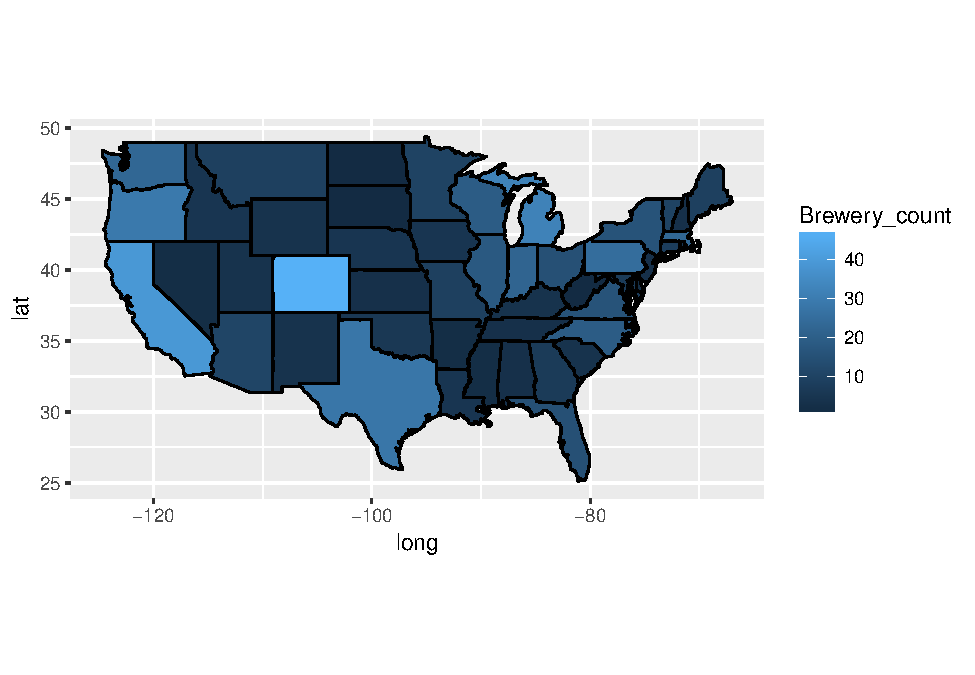
\includegraphics{Analysis_Final_files/figure-latex/unnamed-chunk-7-1.pdf}

\begin{Shaded}
\begin{Highlighting}[]
  \CommentTok{# scale_fill_gradientn(colours = "black",}
  \CommentTok{#                         breaks = c(2, 5, 10, 15, 20, 25, 30, 35, 40, 45, 50))}
\end{Highlighting}
\end{Shaded}

\begin{Shaded}
\begin{Highlighting}[]
\CommentTok{#barplot brewery data by state}
\KeywordTok{ggplot}\NormalTok{(breweries_by_state, }\KeywordTok{aes}\NormalTok{(}\DataTypeTok{x=}\KeywordTok{reorder}\NormalTok{(State, Brewery_count), }\DataTypeTok{y=}\NormalTok{ Brewery_count)) }\OperatorTok{+}\StringTok{  }\CommentTok{#TODO: Make Pretty}
\StringTok{  }\KeywordTok{geom_bar}\NormalTok{(}\DataTypeTok{stat=}\StringTok{"identity"}\NormalTok{) }\OperatorTok{+}
\StringTok{  }\KeywordTok{ylim}\NormalTok{(}\DecValTok{0}\NormalTok{, }\DecValTok{50}\NormalTok{) }\OperatorTok{+}
\StringTok{  }\KeywordTok{theme}\NormalTok{(}\DataTypeTok{text =} \KeywordTok{element_text}\NormalTok{(}\DataTypeTok{size=}\DecValTok{10}\NormalTok{),}
        \DataTypeTok{axis.text.x =} \KeywordTok{element_text}\NormalTok{(}\DataTypeTok{angle=}\DecValTok{90}\NormalTok{, }\DataTypeTok{hjust=}\DecValTok{1}\NormalTok{)) }\OperatorTok{+}
\StringTok{  }\KeywordTok{scale_fill_hue}\NormalTok{(}\DataTypeTok{c=}\DecValTok{45}\NormalTok{, }\DataTypeTok{l=}\DecValTok{40}\NormalTok{, }\DataTypeTok{direction =} \OperatorTok{-}\DecValTok{1}\NormalTok{) }\OperatorTok{+}
\StringTok{  }\KeywordTok{coord_flip}\NormalTok{()}
\end{Highlighting}
\end{Shaded}

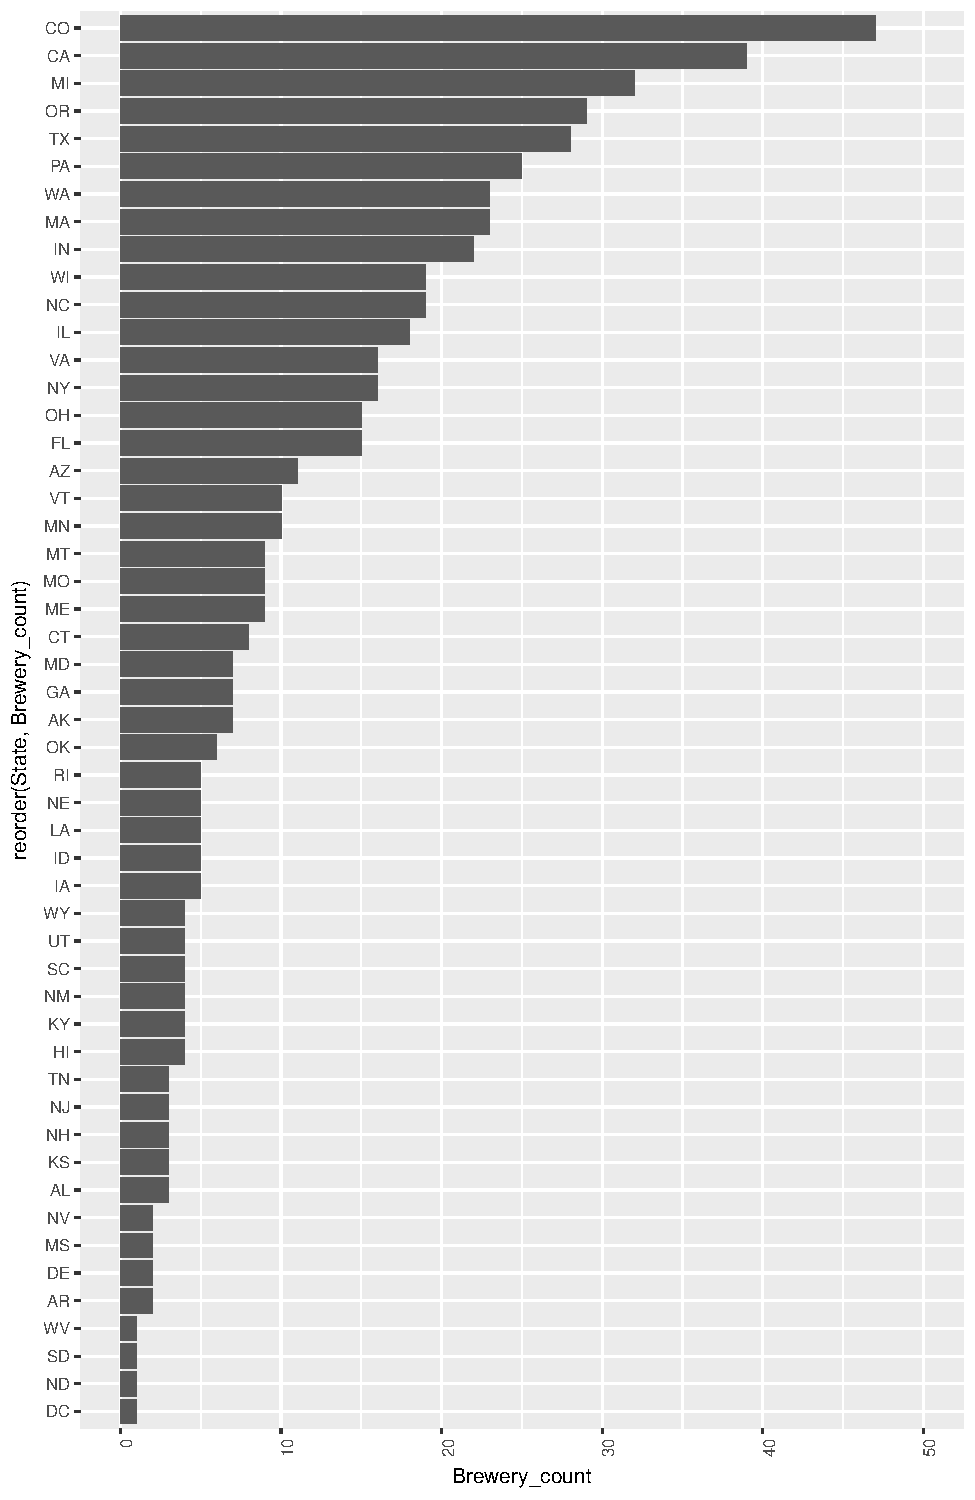
\includegraphics{Analysis_Final_files/figure-latex/unnamed-chunk-8-1.pdf}

\subsection{Question 2}\label{question-2}

\begin{Shaded}
\begin{Highlighting}[]
\CommentTok{# merge beer and breweries}
\NormalTok{merged_data <-}\StringTok{ }\NormalTok{breweries_clean }\OperatorTok
\StringTok{               }\KeywordTok{full_join}\NormalTok{(beer_clean, }\DataTypeTok{by=}\StringTok{"Brew_ID"}\NormalTok{)}


\CommentTok{#TODO: Plot -> brews by brewery}
\end{Highlighting}
\end{Shaded}

\subsection{Question 3}\label{question-3}

\begin{Shaded}
\begin{Highlighting}[]
\CommentTok{# Number of nulls in each column}
\NormalTok{merged_data }\OperatorTok
\StringTok{  }\KeywordTok{select_if}\NormalTok{(}\ControlFlowTok{function}\NormalTok{(x) }\KeywordTok{any}\NormalTok{(}\KeywordTok{is.na}\NormalTok{(x))) }\OperatorTok\StringTok{ }
\StringTok{  }\KeywordTok{summarise_all}\NormalTok{(}\KeywordTok{funs}\NormalTok{(}\KeywordTok{sum}\NormalTok{(}\KeywordTok{is.na}\NormalTok{(.))))}
\end{Highlighting}
\end{Shaded}

\begin{verbatim}
##   ABV  IBU
## 1  62 1005
\end{verbatim}

\begin{Shaded}
\begin{Highlighting}[]
\CommentTok{#TODO: add plot?}
\end{Highlighting}
\end{Shaded}

\subsection{Question 4}\label{question-4}

\begin{Shaded}
\begin{Highlighting}[]
\CommentTok{#fig.width=11}

\CommentTok{# compute median ABV and IBU by state}


\NormalTok{merged_by_state <-}\StringTok{ }\KeywordTok{select}\NormalTok{(merged_data, State, ABV, IBU) }\OperatorTok
\StringTok{                   }\KeywordTok{group_by}\NormalTok{(State) }\OperatorTok
\StringTok{                   }\KeywordTok{summarise_all}\NormalTok{(median)}\CommentTok{#funs(median(!is.na(.)))) #TODO: Double check this is calculating correctly}

\NormalTok{merged_by_state}\OperatorTok{$}\NormalTok{State <-}\StringTok{ }\KeywordTok{as.factor}\NormalTok{(merged_by_state}\OperatorTok{$}\NormalTok{State)  }


\CommentTok{# vars <- rbind(merged_by_state %>% mutate(var="ABV") %>%rename(value=ABV) %>% select(State, var, value),}
\CommentTok{#       merged_by_state %>% mutate(var="IBU") %>%rename(value=IBU) %>% select(State, var, value))}
\CommentTok{# }
\CommentTok{# vars$value}

\KeywordTok{summary}\NormalTok{(merged_by_state)}
\end{Highlighting}
\end{Shaded}

\begin{verbatim}
##      State         ABV               IBU       
##  AK     : 1   Min.   :0.04000   Min.   :32.00  
##  AL     : 1   1st Qu.:0.05400   1st Qu.:33.88  
##  AR     : 1   Median :0.05550   Median :39.75  
##  AZ     : 1   Mean   :0.05514   Mean   :42.25  
##  CA     : 1   3rd Qu.:0.05800   3rd Qu.:48.12  
##  CO     : 1   Max.   :0.06250   Max.   :57.50  
##  (Other):45   NA's   :18        NA's   :47
\end{verbatim}

\begin{Shaded}
\begin{Highlighting}[]
\KeywordTok{kable}\NormalTok{(}\KeywordTok{as.data.frame}\NormalTok{(summarytools}\OperatorTok{::}\KeywordTok{descr}\NormalTok{(beer_clean)),}\DataTypeTok{digits =} \DecValTok{2}\NormalTok{)}
\end{Highlighting}
\end{Shaded}

\begin{longtable}[]{@{}lrrrrr@{}}
\toprule
& Beer\_ID & ABV & IBU & Brew\_ID & Ounces\tabularnewline
\midrule
\endhead
Mean & 1431.11 & 0.06 & 42.71 & 1772.99 & 13.59\tabularnewline
Std.Dev & 752.46 & 0.01 & 25.95 & 31761.76 & 2.35\tabularnewline
Min & 1.00 & 0.00 & 4.00 & 1.00 & 8.40\tabularnewline
Median & 1453.50 & 0.06 & 35.00 & 207.00 & 12.00\tabularnewline
Max & 2692.00 & 0.13 & 138.00 & 697225.00 & 32.00\tabularnewline
MAD & 934.78 & 0.01 & 25.20 & 194.22 & 0.00\tabularnewline
IQR & 1267.50 & 0.02 & 43.00 & 273.50 & 4.00\tabularnewline
CV & 1.90 & 4.41 & 1.65 & 0.06 & 5.78\tabularnewline
Skewness & -0.12 & 0.96 & 0.79 & 21.78 & 2.04\tabularnewline
SE.Skewness & 0.05 & 0.05 & 0.07 & 0.05 & 0.05\tabularnewline
Kurtosis & -1.09 & 1.14 & -0.14 & 473.88 & 9.01\tabularnewline
N.Valid & 2410.00 & 2348.00 & 1405.00 & 2410.00 & 2410.00\tabularnewline
Pct.Valid & 100.00 & 97.43 & 58.30 & 100.00 & 100.00\tabularnewline
\bottomrule
\end{longtable}

\begin{Shaded}
\begin{Highlighting}[]
\NormalTok{merged_by_state }\OperatorTok\StringTok{ }\KeywordTok{na.omit}\NormalTok{(IBU)}
\end{Highlighting}
\end{Shaded}

\begin{verbatim}
## # A tibble: 4 x 3
##   State     ABV   IBU
##   <fctr>  <dbl> <dbl>
## 1 MS     0.0580  45.0
## 2 ND     0.0500  32.0
## 3 NJ     0.0460  34.5
## 4 WV     0.0620  57.5
\end{verbatim}

\begin{Shaded}
\begin{Highlighting}[]
\CommentTok{#MEDIAN}

\KeywordTok{ggplot}\NormalTok{(merged_by_state, }\KeywordTok{aes}\NormalTok{(}\DataTypeTok{x=}\NormalTok{State, }\DataTypeTok{y=}\NormalTok{ABV)) }\OperatorTok{+}
\StringTok{  }\KeywordTok{geom_bar}\NormalTok{(}\DataTypeTok{stat =} \StringTok{"identity"}\NormalTok{, }\DataTypeTok{position =} \StringTok{"dodge"}\NormalTok{) }\OperatorTok{+}
\StringTok{  }\KeywordTok{ylim}\NormalTok{(}\DecValTok{0}\NormalTok{, .}\DecValTok{075}\NormalTok{) }\OperatorTok{+}
\StringTok{  }\KeywordTok{theme}\NormalTok{(}\DataTypeTok{text =} \KeywordTok{element_text}\NormalTok{(}\DataTypeTok{size=}\DecValTok{10}\NormalTok{),}
        \DataTypeTok{axis.text.x =} \KeywordTok{element_text}\NormalTok{(}\DataTypeTok{angle=}\DecValTok{90}\NormalTok{, }\DataTypeTok{hjust=}\DecValTok{1}\NormalTok{)) }
\end{Highlighting}
\end{Shaded}

\begin{verbatim}
## Warning: Removed 18 rows containing missing values (geom_bar).
\end{verbatim}

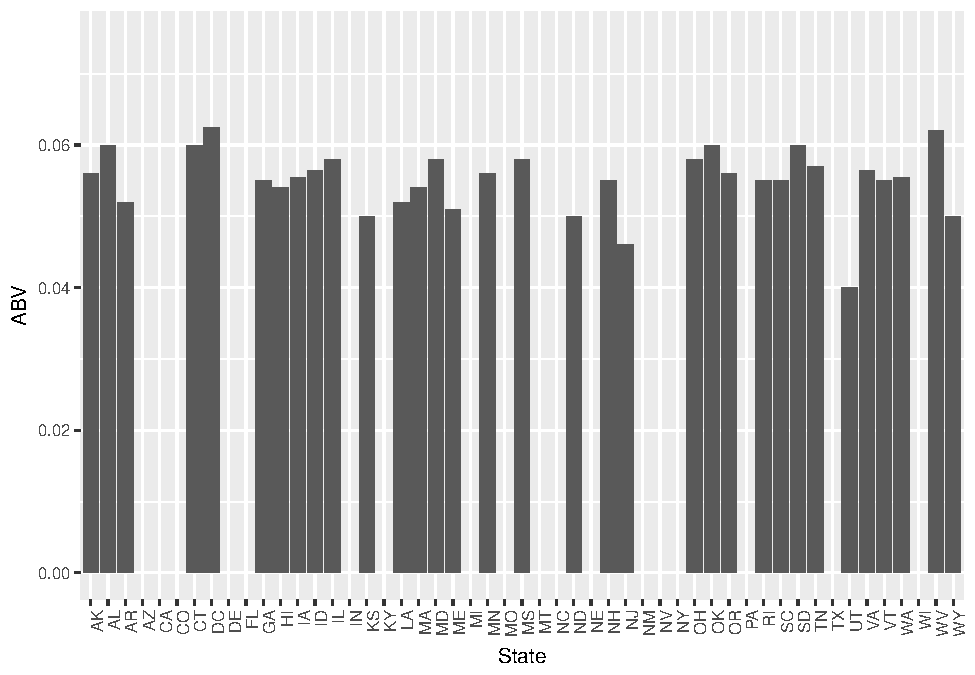
\includegraphics{Analysis_Final_files/figure-latex/unnamed-chunk-11-1.pdf}

\begin{Shaded}
\begin{Highlighting}[]
\KeywordTok{ggplot}\NormalTok{((merged_by_state }\OperatorTok\StringTok{ }\KeywordTok{na.omit}\NormalTok{()), }\KeywordTok{aes}\NormalTok{(}\DataTypeTok{x=}\NormalTok{State, }\DataTypeTok{y=}\NormalTok{IBU)) }\OperatorTok{+}\StringTok{ }\CommentTok{#TODO: something is fishy with IBU}
\StringTok{  }\KeywordTok{geom_bar}\NormalTok{(}\DataTypeTok{stat =} \StringTok{"identity"}\NormalTok{, }\DataTypeTok{position =} \StringTok{"dodge"}\NormalTok{) }\OperatorTok{+}
\StringTok{  }\CommentTok{#ylim(0, .075) +}
\StringTok{  }\KeywordTok{theme}\NormalTok{(}\DataTypeTok{text =} \KeywordTok{element_text}\NormalTok{(}\DataTypeTok{size=}\DecValTok{10}\NormalTok{),}
        \DataTypeTok{axis.text.x =} \KeywordTok{element_text}\NormalTok{(}\DataTypeTok{angle=}\DecValTok{90}\NormalTok{, }\DataTypeTok{hjust=}\DecValTok{1}\NormalTok{)) }
\end{Highlighting}
\end{Shaded}

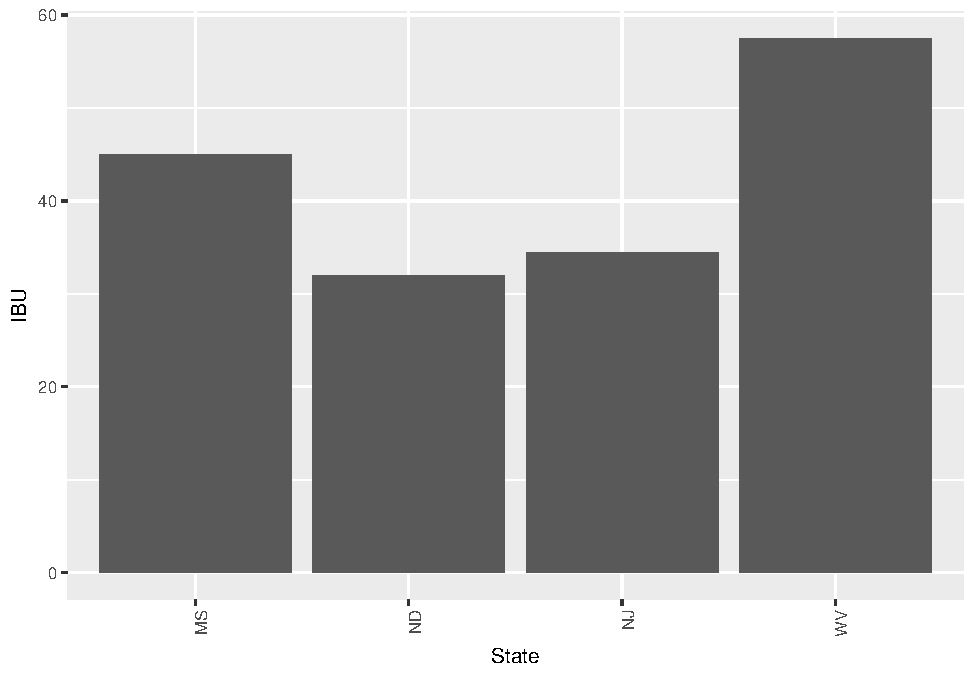
\includegraphics{Analysis_Final_files/figure-latex/unnamed-chunk-11-2.pdf}

\subsection{Question 5}\label{question-5}

\begin{Shaded}
\begin{Highlighting}[]
\CommentTok{# max_abv <- max(merged_data$ABV, na.rm = TRUE)}
  

\KeywordTok{ggplot}\NormalTok{(merged_data, }\KeywordTok{aes}\NormalTok{(}\DataTypeTok{x=}\NormalTok{State , }\DataTypeTok{y=}\NormalTok{ABV)) }\OperatorTok{+}\StringTok{  }\CommentTok{#TODO: Make Pretty}
\StringTok{  }\KeywordTok{geom_boxplot}\NormalTok{() }\OperatorTok{+}
\StringTok{  }\CommentTok{#ylim(0, .075) +}
\StringTok{  }\KeywordTok{theme}\NormalTok{(}\DataTypeTok{text =} \KeywordTok{element_text}\NormalTok{(}\DataTypeTok{size=}\DecValTok{10}\NormalTok{),}
        \DataTypeTok{axis.text.x =} \KeywordTok{element_text}\NormalTok{(}\DataTypeTok{angle=}\DecValTok{90}\NormalTok{, }\DataTypeTok{hjust=}\DecValTok{1}\NormalTok{)) }
\end{Highlighting}
\end{Shaded}

\begin{verbatim}
## Warning: Removed 62 rows containing non-finite values (stat_boxplot).
\end{verbatim}

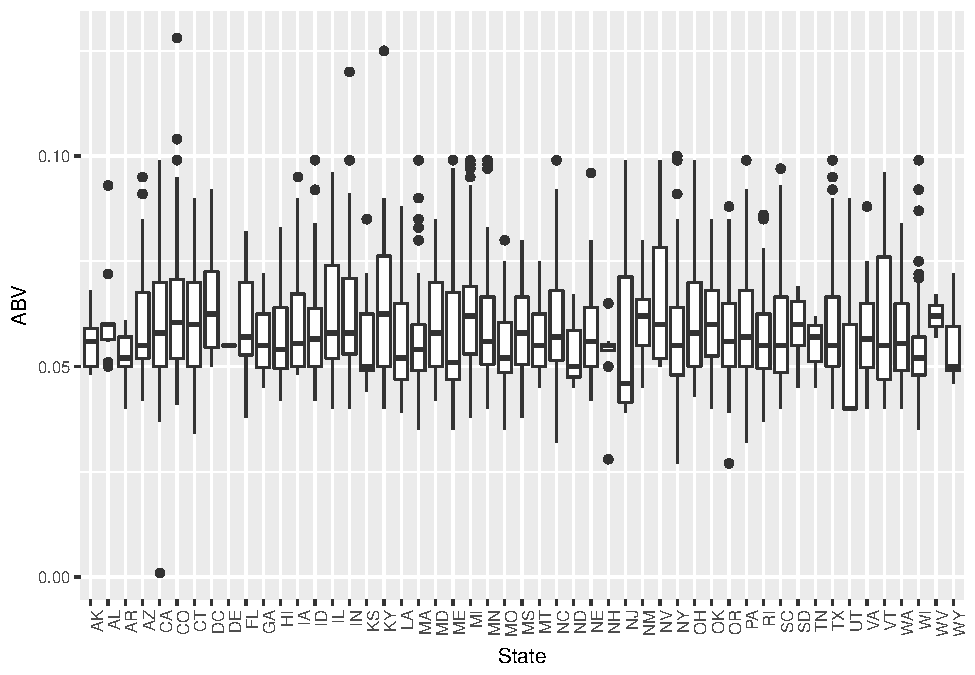
\includegraphics{Analysis_Final_files/figure-latex/unnamed-chunk-12-1.pdf}

\begin{Shaded}
\begin{Highlighting}[]
\KeywordTok{ggplot}\NormalTok{(merged_data, }\KeywordTok{aes}\NormalTok{(}\DataTypeTok{x=}\NormalTok{State , }\DataTypeTok{y=}\NormalTok{IBU)) }\OperatorTok{+}\StringTok{  }\CommentTok{#TODO: Make Pretty}
\StringTok{  }\KeywordTok{geom_boxplot}\NormalTok{() }\OperatorTok{+}
\StringTok{  }\CommentTok{#ylim(0, .075) +}
\StringTok{  }\KeywordTok{theme}\NormalTok{(}\DataTypeTok{text =} \KeywordTok{element_text}\NormalTok{(}\DataTypeTok{size=}\DecValTok{10}\NormalTok{),}
        \DataTypeTok{axis.text.x =} \KeywordTok{element_text}\NormalTok{(}\DataTypeTok{angle=}\DecValTok{90}\NormalTok{, }\DataTypeTok{hjust=}\DecValTok{1}\NormalTok{)) }
\end{Highlighting}
\end{Shaded}

\begin{verbatim}
## Warning: Removed 1005 rows containing non-finite values (stat_boxplot).
\end{verbatim}

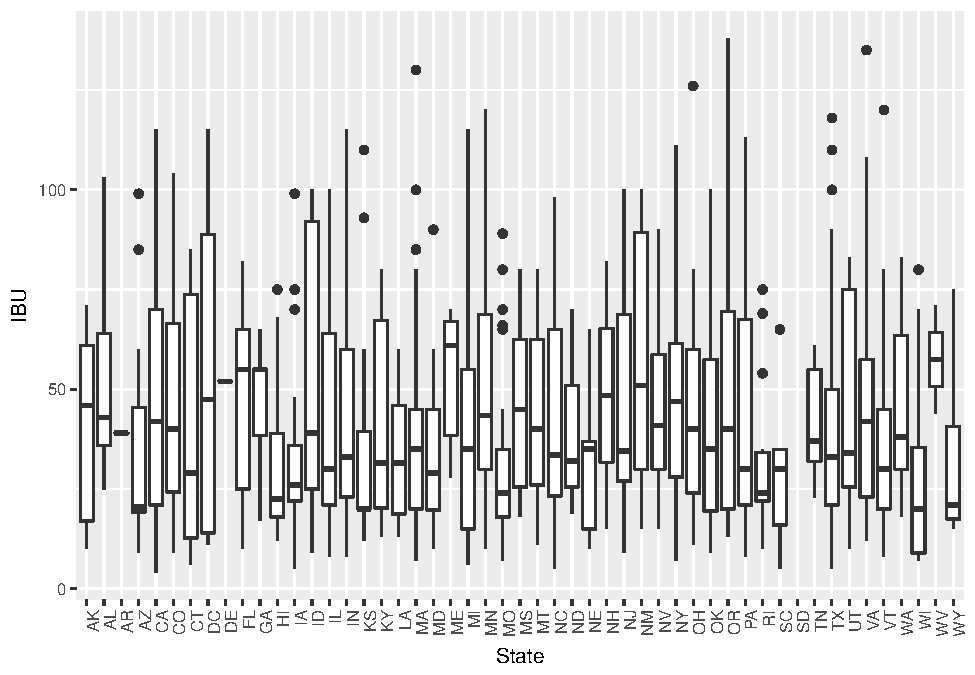
\includegraphics{Analysis_Final_files/figure-latex/unnamed-chunk-12-2.pdf}

\begin{Shaded}
\begin{Highlighting}[]
\NormalTok{max_abv <-}\StringTok{  }\NormalTok{(}\KeywordTok{select}\NormalTok{(merged_data, State, ABV) }\OperatorTok
\StringTok{                   }\KeywordTok{group_by}\NormalTok{(State) }\OperatorTok
\StringTok{                   }\CommentTok{#filter(ABV == max(ABV)) %>%}
\StringTok{                   }\KeywordTok{arrange}\NormalTok{(}\KeywordTok{desc}\NormalTok{(ABV))  }\OperatorTok\StringTok{ }\CommentTok{#sort by ABV}
\StringTok{                   }\KeywordTok{filter}\NormalTok{(}\KeywordTok{row_number}\NormalTok{() }\OperatorTok{==}\StringTok{ }\DecValTok{1}\NormalTok{))[}\DecValTok{1}\NormalTok{,] }\CommentTok{#get first row}
          
\NormalTok{max_abv}
\end{Highlighting}
\end{Shaded}

\begin{verbatim}
## # A tibble: 1 x 2
## # Groups: State [1]
##   State   ABV
##   <chr> <dbl>
## 1 CO    0.128
\end{verbatim}

\begin{Shaded}
\begin{Highlighting}[]
\NormalTok{max_ibu <-}\StringTok{  }\NormalTok{(}\KeywordTok{select}\NormalTok{(merged_data, State, IBU) }\OperatorTok
\StringTok{                   }\KeywordTok{group_by}\NormalTok{(State) }\OperatorTok
\StringTok{                   }\CommentTok{#filter(ABV == max(ABV)) %>%}
\StringTok{                   }\KeywordTok{arrange}\NormalTok{(}\KeywordTok{desc}\NormalTok{(IBU))  }\OperatorTok\StringTok{ }\CommentTok{#sort by ABV}
\StringTok{                   }\KeywordTok{filter}\NormalTok{(}\KeywordTok{row_number}\NormalTok{() }\OperatorTok{==}\StringTok{ }\DecValTok{1}\NormalTok{))[}\DecValTok{1}\NormalTok{,] }\CommentTok{#get first row}
          
\NormalTok{max_ibu}
\end{Highlighting}
\end{Shaded}

\begin{verbatim}
## # A tibble: 1 x 2
## # Groups: State [1]
##   State   IBU
##   <chr> <int>
## 1 OR      138
\end{verbatim}

\subsection{Question 6}\label{question-6}

\begin{Shaded}
\begin{Highlighting}[]
\CommentTok{#summaryize ABV}

\CommentTok{# tidy_summary <- tidy(summary(merged_data$ABV)) #For some reason this line wont knit}


\NormalTok{abv_stats <-}\StringTok{ }\KeywordTok{as.data.frame}\NormalTok{(}\KeywordTok{t}\NormalTok{(}\KeywordTok{summary}\NormalTok{(merged_data}\OperatorTok{$}\NormalTok{ABV))) }\OperatorTok\StringTok{ }\CommentTok{#summarize and transpose}
\StringTok{             }\KeywordTok{rename}\NormalTok{(}\StringTok{"ABV"}\NormalTok{=Freq, }\DataTypeTok{Statistic=}\NormalTok{Var2) }\OperatorTok
\StringTok{             }\KeywordTok{select}\NormalTok{(Statistic, ABV)}

\NormalTok{abv_stats}\OperatorTok{$}\NormalTok{ABV <-}\StringTok{ }\KeywordTok{round}\NormalTok{(abv_stats}\OperatorTok{$}\NormalTok{ABV, }\DataTypeTok{digits =} \DecValTok{3}\NormalTok{)}
  

\NormalTok{abv_stats }\CommentTok{#TODO: Add IQR, stdev    #TODO: Compare to quinton's summary}
\end{Highlighting}
\end{Shaded}

\begin{verbatim}
##   Statistic    ABV
## 1      Min.  0.001
## 2   1st Qu.  0.050
## 3    Median  0.056
## 4      Mean  0.060
## 5   3rd Qu.  0.067
## 6      Max.  0.128
## 7      NA's 62.000
\end{verbatim}

\subsection{Question 7}\label{question-7}

\begin{Shaded}
\begin{Highlighting}[]
\CommentTok{# fig.height=48}
\CommentTok{#plot relationshiop of ABV and IBU}

\CommentTok{#retreive linear model equation -- source(https://stackoverflow.com/questions/7549694/adding-regression-line-equation-and-r2-on-graph)}
\NormalTok{lm_eqn =}\StringTok{ }\ControlFlowTok{function}\NormalTok{(m) \{}

\NormalTok{  l <-}\StringTok{ }\KeywordTok{list}\NormalTok{(}\DataTypeTok{a =} \KeywordTok{format}\NormalTok{(}\KeywordTok{coef}\NormalTok{(m)[}\DecValTok{1}\NormalTok{], }\DataTypeTok{digits =} \DecValTok{2}\NormalTok{),}
      \DataTypeTok{b =} \KeywordTok{format}\NormalTok{(}\KeywordTok{abs}\NormalTok{(}\KeywordTok{coef}\NormalTok{(m)[}\DecValTok{2}\NormalTok{]), }\DataTypeTok{digits =} \DecValTok{2}\NormalTok{),}
      \DataTypeTok{r2 =} \KeywordTok{format}\NormalTok{(}\KeywordTok{summary}\NormalTok{(m)}\OperatorTok{$}\NormalTok{r.squared, }\DataTypeTok{digits =} \DecValTok{3}\NormalTok{));}

  \ControlFlowTok{if}\NormalTok{ (}\KeywordTok{coef}\NormalTok{(m)[}\DecValTok{2}\NormalTok{] }\OperatorTok{>=}\StringTok{ }\DecValTok{0}\NormalTok{)  \{}
\NormalTok{    eq <-}\StringTok{ }\KeywordTok{substitute}\NormalTok{(}\KeywordTok{italic}\NormalTok{(y) }\OperatorTok{==}\StringTok{ }\NormalTok{a }\OperatorTok{+}\StringTok{ }\NormalTok{b }\OperatorTok\StringTok{ }\KeywordTok{italic}\NormalTok{(x)}\OperatorTok{*}\StringTok{","}\OperatorTok{~}\ErrorTok{~}\KeywordTok{italic}\NormalTok{(r)}\OperatorTok{^}\DecValTok{2}\OperatorTok{~}\StringTok{"="}\OperatorTok{~}\NormalTok{r2,l)}
\NormalTok{  \} }\ControlFlowTok{else}\NormalTok{ \{}
\NormalTok{    eq <-}\StringTok{ }\KeywordTok{substitute}\NormalTok{(}\KeywordTok{italic}\NormalTok{(y) }\OperatorTok{==}\StringTok{ }\NormalTok{a }\OperatorTok{-}\StringTok{ }\NormalTok{b }\OperatorTok\StringTok{ }\KeywordTok{italic}\NormalTok{(x)}\OperatorTok{*}\StringTok{","}\OperatorTok{~}\ErrorTok{~}\KeywordTok{italic}\NormalTok{(r)}\OperatorTok{^}\DecValTok{2}\OperatorTok{~}\StringTok{"="}\OperatorTok{~}\NormalTok{r2,l)    }
\NormalTok{  \}}

  \KeywordTok{as.character}\NormalTok{(}\KeywordTok{as.expression}\NormalTok{(eq));                 }
\NormalTok{\}}
\KeywordTok{ggplot}\NormalTok{(beer_clean, }\KeywordTok{aes}\NormalTok{(}\DataTypeTok{x=}\NormalTok{ABV, }\DataTypeTok{y=}\NormalTok{IBU)) }\OperatorTok{+}
\StringTok{  }\KeywordTok{geom_point}\NormalTok{() }\OperatorTok{+}
\StringTok{  }\KeywordTok{geom_smooth}\NormalTok{(}\DataTypeTok{method =} \StringTok{"lm"}\NormalTok{) }\OperatorTok{+}
\StringTok{  }\KeywordTok{geom_text}\NormalTok{(}\KeywordTok{aes}\NormalTok{(}\DataTypeTok{x =}\NormalTok{ .}\DecValTok{02}\NormalTok{, }\DataTypeTok{y =} \DecValTok{100}\NormalTok{, }\DataTypeTok{label =} \KeywordTok{lm_eqn}\NormalTok{(}\KeywordTok{lm}\NormalTok{(ABV }\OperatorTok{~}\StringTok{ }\NormalTok{IBU ,beer_clean))), }\DataTypeTok{parse =} \OtherTok{TRUE}\NormalTok{, }\DataTypeTok{color =} \StringTok{"red"}\NormalTok{)}
\end{Highlighting}
\end{Shaded}

\begin{verbatim}
## Warning: Removed 1005 rows containing non-finite values (stat_smooth).
\end{verbatim}

\begin{verbatim}
## Warning: Removed 1005 rows containing missing values (geom_point).
\end{verbatim}

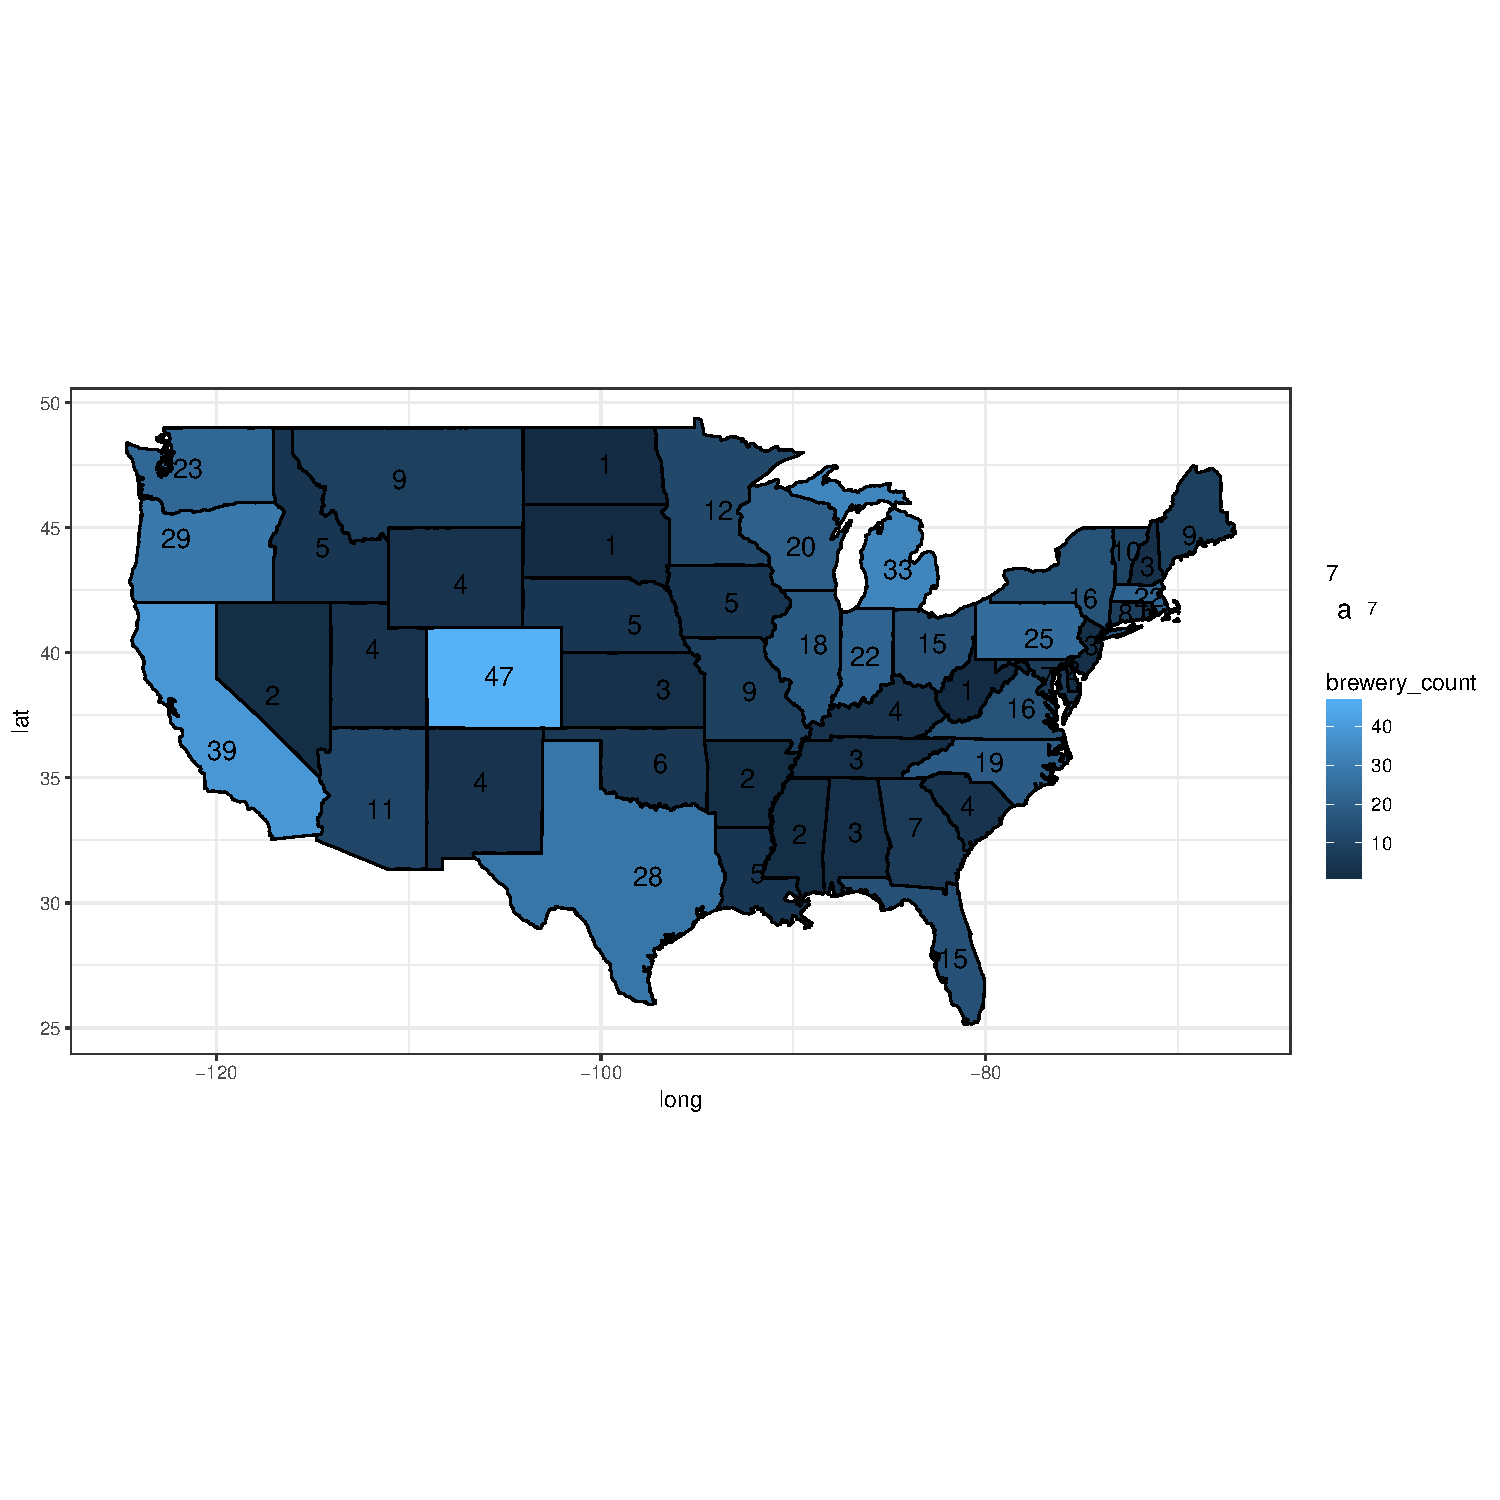
\includegraphics{Analysis_Final_files/figure-latex/unnamed-chunk-14-1.pdf}

\begin{Shaded}
\begin{Highlighting}[]
\CommentTok{# Yes, there is a positive relationship between ABV and IBU. #TODO:Add explanation}
\end{Highlighting}
\end{Shaded}

\subsection{Appendex}\label{appendex}

\paragraph{Session Info}\label{session-info}

\begin{Shaded}
\begin{Highlighting}[]
\KeywordTok{sessionInfo}\NormalTok{()}
\end{Highlighting}
\end{Shaded}

\begin{verbatim}
## R version 3.4.3 (2017-11-30)
## Platform: x86_64-w64-mingw32/x64 (64-bit)
## Running under: Windows 10 x64 (build 16299)
## 
## Matrix products: default
## 
## locale:
## [1] LC_COLLATE=English_United States.1252 
## [2] LC_CTYPE=English_United States.1252   
## [3] LC_MONETARY=English_United States.1252
## [4] LC_NUMERIC=C                          
## [5] LC_TIME=English_United States.1252    
## 
## attached base packages:
## [1] stats     graphics  grDevices utils     datasets  methods   base     
## 
## other attached packages:
##  [1] bindrcpp_0.2         stargazer_5.2        magrittr_1.5        
##  [4] summarytools_0.8.0   RColorBrewer_1.1-2   maps_3.2.0          
##  [7] ggplot2_2.2.1        knitr_1.18           tidyr_0.7.2         
## [10] dplyr_0.7.4          RevoUtilsMath_10.0.1 RevoUtils_10.0.7    
## [13] RevoMods_11.0.0      MicrosoftML_9.3.0    mrsdeploy_1.1.3     
## [16] RevoScaleR_9.3.0     lattice_0.20-35      rpart_4.1-11        
## 
## loaded via a namespace (and not attached):
##  [1] purrr_0.2.4            pander_0.6.1           colorspace_1.3-2      
##  [4] htmltools_0.3.6        yaml_2.1.16            CompatibilityAPI_1.1.0
##  [7] utf8_1.1.2             rlang_0.1.6            pillar_1.0.1          
## [10] glue_1.2.0             pryr_0.1.3             matrixStats_0.52.2    
## [13] foreach_1.4.5          bindr_0.1              plyr_1.8.4            
## [16] stringr_1.2.0          munsell_0.4.3          gtable_0.2.0          
## [19] codetools_0.2-15       evaluate_0.10.1        labeling_0.3          
## [22] curl_3.1               highr_0.6              Rcpp_0.12.14          
## [25] scales_0.5.0           backports_1.1.2        jsonlite_1.5          
## [28] rapportools_1.0        digest_0.6.13          stringi_1.1.6         
## [31] grid_3.4.3             rprojroot_1.3-1        cli_1.0.0             
## [34] tools_3.4.3            bitops_1.0-6           lazyeval_0.2.1        
## [37] RCurl_1.95-4.9         tibble_1.4.1           crayon_1.3.4          
## [40] pkgconfig_2.0.1        assertthat_0.2.0       rmarkdown_1.8         
## [43] iterators_1.0.9        R6_2.2.2               compiler_3.4.3
\end{verbatim}


\end{document}
